\section{Tutorial A10.3}

\begin{problem}
    Given that $z = 1 + \i$ and $w = 1 + 2\i$, mark on an Argand diagram, the positions representing: $z$, $w$, $z + w$, $z - w$, $\i z$ and $2z\conj$.
\end{problem}
\begin{solution}
    \begin{center}\tikzsetnextfilename{73}
        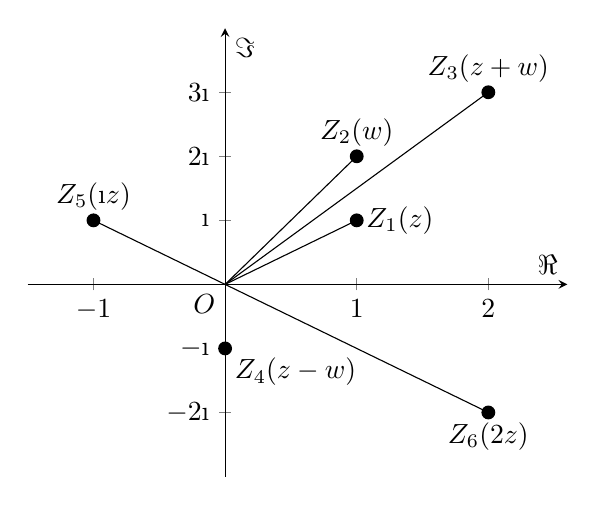
\begin{tikzpicture}[trim axis left, trim axis right]
            \begin{axis}[
                domain = 0:10,
                samples = 101,
                axis y line=middle,
                axis x line=middle,
                xtick = {-1, 1, 2},
                ytick = {-2, -1, 1, 2, 3},
                yticklabels = {$-2\i$, $-\i$, $\i$, $2\i$, $3\i$},
                xmax=2.6,
                xmin=-1.5,
                ymin=-3,
                ymax=4,
                xlabel = {$\Re$},
                ylabel = {$\Im$},
                legend cell align={left},
                legend pos=outer north east,
                after end axis/.code={
                    \path (axis cs:0,0) 
                        node [anchor=north east] {$O$};
                    }
                ]
    
                \coordinate (R) at (10,0);
                \coordinate[label=right:$Z_1(z)$] (Z1) at (1, 1);
                \coordinate[label=above:$Z_2(w)$] (Z2) at (1, 2);
                \coordinate[label=above:$Z_3(z + w)$] (Z3) at (2, 3);
                \coordinate[label=below right:$Z_4(z - w)$] (Z4) at (0, -1);
                \coordinate[label=above:$Z_5(\i z)$] (Z5) at (-1, 1);
                \coordinate[label=below:$Z_6(2z\conj)$] (Z6) at (2, -2);
                \coordinate (O) at (0, 0);
        
                \draw (O) -- (Z1);
                \draw (O) -- (Z2);
                \draw (O) -- (Z3);
                \draw (O) -- (Z4);
                \draw (O) -- (Z5);
                \draw (O) -- (Z6);
        
                \fill (Z1) circle[radius=2.5pt];
                \fill (Z2) circle[radius=2.5pt];
                \fill (Z3) circle[radius=2.5pt];
                \fill (Z4) circle[radius=2.5pt];
                \fill (Z5) circle[radius=2.5pt];
                \fill (Z6) circle[radius=2.5pt];
            \end{axis}
        \end{tikzpicture}
    \end{center}
\end{solution}

\begin{problem}
    \begin{enumerate}
        \item Write down the exact values of the modulus and the argument of the complex number $\frac12 + \frac{\sqrt3}2 \i$.
        \item The complex numbers $z$ and $w$ satisfy the equation \[z^2 - zw + w^2 = 0.\] Find $z$ in terms of $w$. In an Argand diagram, the points $O$, $A$ and $B$ represent the complex numbers $0$, $z$ and $w$ respectively. Show that $\triangle OAB$ is an equilateral triangle.
    \end{enumerate}
\end{problem}
\begin{solution}
    \begin{ppart}
        We have $r^2 = \bp{\frac12}^2 + \bp{\frac{\sqrt3}2}^2 \implies r = 1$ and $\tan \t = \frac{\sqrt3 /2}{1/2} \implies \t = \frac\pi3$. Hence, $\abs{\frac12 + \frac{\sqrt3}2 \i} = 1$ and $\arg{\frac12 + \frac{\sqrt3}2 \i} = \frac\pi3$.
    \end{ppart}
    \begin{ppart}
        From the quadratic formula, we have \[z = \frac{w \pm \sqrt{w^2 - 4w^2}}{2} = w \bp{\frac12 \pm \frac{\sqrt3}2 \i}.\]

            \begin{center}\tikzsetnextfilename{74}
                \begin{tikzpicture}[trim axis left, trim axis right]
                    \begin{axis}[
                        domain = 0:10,
                        samples = 101,
                        axis y line=middle,
                        axis x line=middle,
                        xtick = \empty,
                        ytick = \empty,
                        xmax=2,
                        xmin=-2,
                        ymin=-1.5,
                        ymax=2,
                        xlabel = {$\Re$},
                        ylabel = {$\Im$},
                        legend cell align={left},
                        legend pos=outer north east,
                        after end axis/.code={
                            \path (axis cs:0,0) 
                                node [anchor=north east] {$O$};
                            }
                        ]
            
                        \coordinate (R) at (10,0);
                        \coordinate[label=right:$B(w)$] (B) at (1, 1);
                        \coordinate[label=left:$A_1(z_1)$] (A1) at (-0.366, 1.366);
                        \coordinate[label=below:$A_2(z_2)$] (A2) at (1.366, -0.366);

                        \coordinate (O) at (0, 0);
                
                        \draw (O) -- (B);
                        \draw (O) -- (A1);
                        \draw (O) -- (A2);
                        
                        \draw[dotted] (A1) -- (B);
                        \draw[dotted] (A2) -- (B);
                
                        \fill (A1) circle[radius=2.5pt];
                        \fill (A2) circle[radius=2.5pt];
                        \fill (B) circle[radius=2.5pt];
                        \draw pic [draw, angle radius=10mm, "$\t$"] {angle = B--O--A1};
                        \draw pic [draw, angle radius=12mm, "$\t$"] {angle = A2--O--B};
                    \end{axis}
                \end{tikzpicture}
            \end{center}

            Since $\abs{\frac12 \pm \frac{\sqrt3}2 \i} = 1$, we have that $OB = OA_1 = OA_2$. Further, since $\arg{\frac12 \pm \frac{\sqrt3}2 \i} = \pm \pi/3$, we know $\angle A_1OB = \angle A_2OB = \pi/3$, whence $\triangle A_1OB$ and $\triangle A_2OB$ are both equilateral.
    \end{ppart}
\end{solution}

\begin{problem}
    Find the exact roots of the equations
    \begin{enumerate}
        \item $z^3 = 1$
        \item $(z-1)^4 = -16$
    \end{enumerate}
    in the form $x + \i y$.
\end{problem}
\begin{solution}
    \begin{ppart}
        Note that \[z^3 = 1 = \e^{\i 2\pi n} \implies z = \e^{\i 2 \pi n / 3} = \cos \frac{2\pi n}3 + \i \sin \frac{2\pi n}3,\] for $n \in \ZZ$. Evaluating $z$ in the $n = 0, 1, 2$ cases, we see that the roots of $z^3 = 1$ are \[z = 1, \, -\frac12 + \frac{\sqrt3}2 \i, \, -\frac12 - \frac{\sqrt3}2 \i.\]
    \end{ppart}
    \begin{ppart}
        Note that $(z-1)^4 = -16 = 16\e^{\i \pi (2n + 1)}$. Hence, \[z = 1 + 2\e^{\i\pi (2n + 1)/4} = 1 + 2\bs{\cos{\frac{2n+1}4 \pi} + \i\sin{\frac{2n+1}4 \pi}},\] where $n \in \ZZ$.
        Evaluating $z$ in the $n = 0, 1, 2, 3$ cases, we see that the roots of $(z-1)^4 = -16$ are \[z = (1 + \sqrt2) + \i\sqrt2, \, (1 - \sqrt2) + \i\sqrt2, \, (1 - \sqrt2) - \i\sqrt2, \, (1 + \sqrt2) - \i\sqrt2.\]
    \end{ppart}
\end{solution}

\begin{problem}
    \begin{enumerate}
        \item Write down the 5 roots of the equation $z^5 - 1 = 0$ in the form $r\e^{\i\t}$, where $r > 0$ and $-\pi < \t \leq \pi$.
        \item Show that the roots of the equation $(5+z)^5 - (5-z)^5 = 0$ can be written in the form $5\i \tan \frac{k\pi}5$, where $k = 0, \pm 1, \pm 2.$
    \end{enumerate}
\end{problem}
\begin{solution}
    \begin{ppart}
        Note that \[z^5 = 1 = \e^{\i 2\pi n} \implies z = \e^{\i 2\pi n /5}.\] Since $- \pi < \t \leq \pi$, we have \[z = \e^{-\i 4\pi/5}, \, \e^{-\i 2\pi/5}, \, 1, \, \e^{\i 2\pi/5}, \, \e^{\i 4\pi/5}.\]
    \end{ppart}
    \begin{ppart}
        Note that \[(5+z)^5 - (5-z)^5 = 0 \implies \bp{\frac{5+z}{5-z}}^5 - 1 = 0 \implies \frac{5+z}{5-z} = \e^{\i2k\pi/5}.\] Solving for $z$, we get \[z = 5\bp{\frac{\e^{\i2k\pi/5} - 1}{\e^{\i2k\pi/5} + 1}} = 5\bp{\frac{\e^{\i k\pi/5} - \e^{-\i k\pi/5}}{\e^{\i k\pi/5} + \e^{-\i k\pi/5}}} = 5\bs{\frac{2\i \sin{k\pi/5}}{2\cos{k\pi/5}}} = 5\i\tan \frac{k\pi}5.\]
    \end{ppart}
\end{solution}

\begin{problem}
    De Moivre's theorem for a positive integral exponent states that \[(\cos\t + \i\sin\t)^n = \cos n\t + \i\sin n\t.\] Use de Moivre's theorem to show that \[\cos 7\t = 64 \cos^7 \t - 112 \cos^5 \t + 56 \cos^3 \t - 7 \cos \t.\] Hence, obtain the roots of the equation \[128x^7 - 224x^5 + 112x^3 - 14x + 1 = 0\] in the form $\cos q\pi$, where $q$ is a rational number.
\end{problem}
\begin{solution}
    Taking $n = 7$, we have $\cos 7\t + \i\sin 7\t = (\cos\t + \i\sin\t)^7$, whence $\cos 7\t = \Re (\cos \t + \i\sin \t)^7$. Let $c = \cos \t$ and $s = \sin \t$. By the binomial theorem,  \[\cos 7\t = \Re \, (c + \i s)^7 = \Re \, \sum_{k = 0}^7 \binom{7}{k} \i^k s^k c^{7-k}.\] Note that $\Re i^k$ is given by \[
        \Re i^k = \begin{cases}
            0, &k = 1, 3 \pmod{4}\\
            1, &k = 0 \pmod{4}\\
            -1, &k = 2 \pmod{4}
    \end{cases}\] We hence have
    \begin{gather*}
        \cos 7\t = c^7 - 21c^5s^2 + 35c^3s^4 - 7cs^6 = c^7 - 21c^5\bp{1-c^2} + 35c^3\bp{1 - c^2}^2 - 7c\bp{1 - c^2}^3\\
        = 64c^7 - 112c^5 + 56c^3 - 7c = 64\cos^7\t - 112\cos^5 + 56 \cos^3\t - 7\cos\t.
    \end{gather*}

    Observe that we can manipulate the given equation into \[128x^7 - 224x^5 + 112x^3 - 14x + 1 = 0 \implies 64x^7 - 112x^5 + 56x^3 - 7x = -\frac12.\] Under the substitution $x = \cos \t$, we see that \[\cos 7\t = -\frac12 \implies 7\t = \frac23 \pi + 2\pi n \implies \t = \frac{2\pi}{21} (3n + 1),\] where $n \in \ZZ$. Taking $0 \leq n < 7$,
    \begin{align*}
        x &= \cos \frac{2\pi}{21}, \, \cos \frac{8\pi}{21}, \, \cos \frac{14\pi}{21}, \, \cos \frac{20\pi}{21}, \, \cos \frac{26\pi}{21}, \, \cos \frac{32\pi}{21}, \, \cos \frac{38\pi}{21}\\
        &= \cos \frac{2\pi}{21}, \, \cos \frac{4\pi}{21}, \, \cos \frac{8\pi}{21}, \, \cos \frac{10\pi}{21}, \, \cos \frac{14\pi}{21}, \, \cos \frac{16\pi}{21}, \, \cos \frac{20\pi}{21}.
    \end{align*}
\end{solution}

\begin{problem}
    By considering $\sum_{n=1}^N z^{2n-1}$, where $z = \e^{\i\t}$, or by any method, show that \[\sum_{n=1}^N \sin (2n-1)\t = \frac{\sin^2 N\t}{\sin \t},\] provided $\sin \t \neq 0$.
\end{problem}
\begin{solution}
    Observe that \[\sum_{n=1}^N \sin(2n-1)\t = \Im \sum_{n=1}^N \bs{\cos(2n-1)\t + \i\sin(2n-1)\t} = \Im \sum_{n=1}^N z^{2n-1}.\] Since
    \begin{gather*}
        \sum_{n=1}^N z^{2n-1} = \frac1z \sum_{n=1}^N \bp{z^2}^n = \frac1z \bp{\frac{z^2 \bs{\bp{z^2}^N - 1}}{z^2 - 1}} = \frac{z^{2N} - 1}{z - z^{-1}}\\
        = z^N \bp{\frac{z^N - z^{-N}}{z - z^{-1}}} = z^N \bp{\frac{2\i \sin N\t}{2\i \sin \t}} = z^N \bp{\frac{\sin N\t}{\sin \t}},
    \end{gather*}
    we have \[\sum_{n=1}^N \sin(2n-1)\t = \bp{\frac{\sin N\t}{\sin \t}}\Im{z^N} = \bp{\frac{\sin N\t}{\sin \t}} \sin N\t = \frac{\sin^2 N\t}{\sin \t}.\]
\end{solution}

\begin{problem}
    By considering the series $\sum_{n=0}^N \bp{\e^{2\i\t}}^n$, show that, provided $\sin \t \neq 0$, \[\sum_{n = 0}^N \cos 2n\t = \frac{\sin(N+1)\t \cos N\t}{\sin \t}\] and deduce that \[\sum_{n = 0}^N \sin^2 n\t = \frac{N}2 + \frac12 - \frac{\sin(N+1)\t \cos N\t}{2\sin\t}.\]
\end{problem}
\begin{solution}
    Let $z = \e^{\i\t}$. Then \[\sum_{n = 0}^N \cos 2n\t = \Re \sum_{n = 0}^N \bp{\cos 2n\t + \i\sin 2n\t} = \Re \sum_{n=0}^{N} \e^{\i2n\t} = \Re \sum_{n=0}^{N} \bp{z^2}^n.\] Observe that \[\sum_{n=0}^{N} \bp{z^2}^n = \frac{\bp{z^2}^{N+1} - 1}{z^2 - 1} = \frac{z^{N+1}}{z} \bp{\frac{z^{N+1} - z^{-(N+1)}}{z - z^{-1}}} = z^N \bp{\frac{\sin (N+1)\t}{\sin \t}}.\] Hence, \[\sum_{n = 0}^N \cos 2n\t = \bp{\frac{\sin (N+1)\t}{\sin \t}} \Re{z^N} = \frac{\sin(N+1)\t \cos N\t}{\sin \t}.\]

    Recall that $\cos 2n\t = 1 - 2\sin^2 n\t \implies \sin^2 n\t = \frac12 (1 - 2\cos 2n\t)$. Thus, \[\sum_{n = 0}^N \sin^2 n\t = \frac12 \sum_{n = 0}^N (1 - \cos 2n\t) = \frac{N + 1}2 - \frac{\sin(N+1)\t \cos N\t}{2\sin\t}.\]
\end{solution}

\begin{problem}
    Given that $z = \e^{\i\t}$, show that $z^k + 1/{z^k} = 2\cos k\t$, $k \in \ZZ$.

    Hence, show that $\cos^8 \t = \frac1{128} \bp{\cos 8\t + 8\cos6\t + 28\cos4\t + 56\cos2\t + 35}$.

    Find, correct to three decimal places, the values of $\t$ such that $0 < \t < \frac12 \pi$ and $\cos 8\t + 8\cos6\t + 28\cos4\t + 56\cos2\t + 1 = 0$.
\end{problem}
\begin{solution}
    Note that
    \begin{gather*}
        z^k + \frac1{z^k} = z^k + z^{-k} = \bp{\e^{\i\t}}^k + \bp{\e^{\i \t}}^{-k} = \e^{\i k \t} + \e^{-\i k \t}\\
        = \bs{\cos{k\t} + \i\sin{k\t}} + \bs{\cos{-k\t} + \i\sin{-k\t}} = 2\cos{k\t}.
    \end{gather*}

    Observe that
    \begin{gather*}
        \cos^8 \t = \frac1{256} (2\cos \t)^8 = \frac1{256} (z + z^{-1})^8 = \frac1{256} z^{-8} \bp{z^2 + 1}^8\\
        = \frac1{256} \bp{z^{-8} + 8z^{-6} + 28z^{-4} + 56z^{-2} + 70 + 56z^2 + 28z^4 + 8z^6 + z^8}\\
        = \frac1{128} \bs{\bp{\frac{z^8 + z^{-8}}2} + 8\bp{\frac{z^6 + z^{-6}}2} + 28\bp{\frac{z^4 + z^{-4}}2} + 56\bp{\frac{z^2 + z^{-2}}2} + \frac{70}2}\\
        = \frac1{128} \bp{\cos 8\t + 8\cos 6\t + 28\cos 4\t + 56\cos 2\t + 35}.
    \end{gather*}

    Note that we rewrite the equation as \[\cos 8\t + 8\cos6\t + 28\cos4\t + 56\cos2\t + 35 = 128\cos^8\t = 34.\] Thus, \[\cos\t = \sqrt[8]{\frac{34}{128}} \implies \t = 0.560 \tosf{3}.\]
\end{solution}